\documentclass{standalone}
\usepackage{tikz}
\usetikzlibrary{patterns, positioning}


\begin{document}
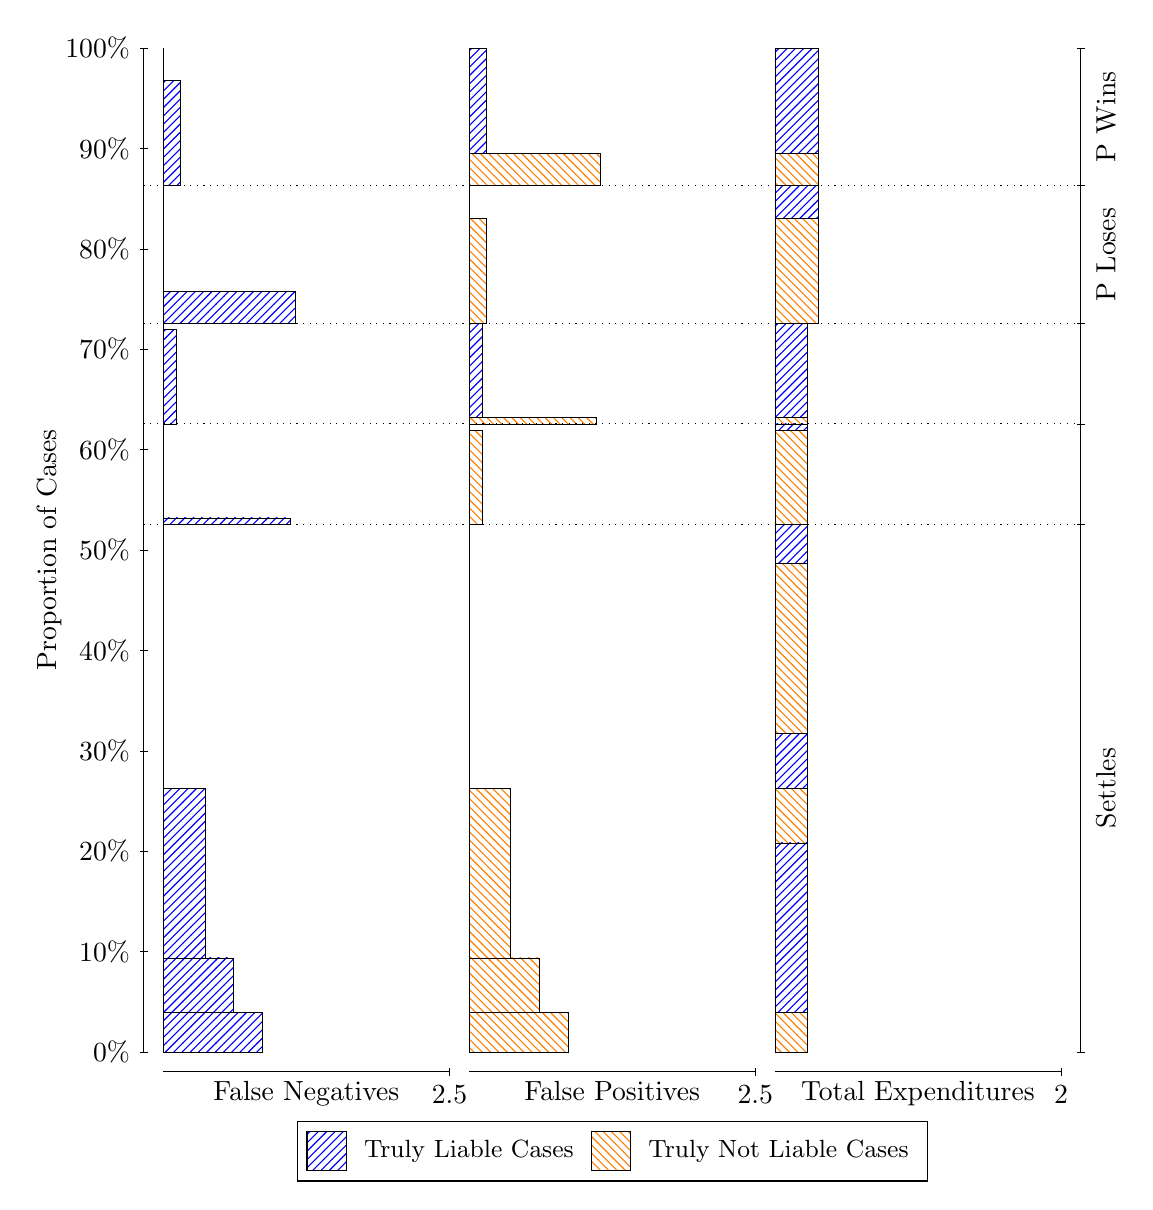
\begin{tikzpicture}
\draw[black, very thin] (1.5,1.75) -- (1.5,14.5);
\node[rotate=90, text=black, anchor=center] at (0.3, 8.125) {Proportion of Cases};
\draw[black, very thin] (1.45,1.75) -- (1.55,1.75);
\node[text=black, anchor=east] at (1.45, 1.75) {0\%};
\draw[black, very thin] (1.45,3.025) -- (1.55,3.025);
\node[text=black, anchor=east] at (1.45, 3.025) {10\%};
\draw[black, very thin] (1.45,4.3) -- (1.55,4.3);
\node[text=black, anchor=east] at (1.45, 4.3) {20\%};
\draw[black, very thin] (1.45,5.575) -- (1.55,5.575);
\node[text=black, anchor=east] at (1.45, 5.575) {30\%};
\draw[black, very thin] (1.45,6.85) -- (1.55,6.85);
\node[text=black, anchor=east] at (1.45, 6.85) {40\%};
\draw[black, very thin] (1.45,8.125) -- (1.55,8.125);
\node[text=black, anchor=east] at (1.45, 8.125) {50\%};
\draw[black, very thin] (1.45,9.4) -- (1.55,9.4);
\node[text=black, anchor=east] at (1.45, 9.4) {60\%};
\draw[black, very thin] (1.45,10.675) -- (1.55,10.675);
\node[text=black, anchor=east] at (1.45, 10.675) {70\%};
\draw[black, very thin] (1.45,11.95) -- (1.55,11.95);
\node[text=black, anchor=east] at (1.45, 11.95) {80\%};
\draw[black, very thin] (1.45,13.225) -- (1.55,13.225);
\node[text=black, anchor=east] at (1.45, 13.225) {90\%};
\draw[black, very thin] (1.45,14.5) -- (1.55,14.5);
\node[text=black, anchor=east] at (1.45, 14.5) {100\%};

\draw[black, very thin] (13.4,1.75) -- (13.4,14.5);
\draw[black, very thin] (13.35,1.75) -- (13.45,1.75);
\node[anchor=west] at (13.35, 1.75) {};
\draw[black, very thin] (13.35,8.4523) -- (13.45,8.4523);
\node[anchor=west] at (13.35, 8.4523) {};
\draw[black, very thin] (13.35,9.7273) -- (13.45,9.7273);
\node[anchor=west] at (13.35, 9.7273) {};
\draw[black, very thin] (13.35,11.002) -- (13.45,11.002);
\node[anchor=west] at (13.35, 11.002) {};
\draw[black, very thin] (13.35,12.751) -- (13.45,12.751);
\node[anchor=west] at (13.35, 12.751) {};
\draw[black, very thin] (13.35,14.5) -- (13.45,14.5);
\node[anchor=west] at (13.35, 14.5) {};

\draw[black, very thin, pattern color=blue, pattern=north east lines] (1.75,1.75) rectangle (3.0035,2.251);
\draw[black, very thin, pattern color=blue, pattern=north east lines] (1.75,2.251) rectangle (2.6402,2.9462);
\draw[black, very thin, pattern color=blue, pattern=north east lines] (1.75,2.9462) rectangle (2.2768,5.1012);
\draw[black, very thin, pattern color=orange, pattern=north west lines] (1.75,5.1012) rectangle (1.75,8.4523);
\draw[black, very thin, pattern color=blue, pattern=north east lines] (1.75,8.4523) rectangle (3.3668,8.5315);
\draw[black, very thin, pattern color=orange, pattern=north west lines] (1.75,8.5315) rectangle (1.75,9.7273);
\draw[black, very thin, pattern color=blue, pattern=north east lines] (1.75,9.7273) rectangle (1.9135,10.923);
\draw[black, very thin, pattern color=orange, pattern=north west lines] (1.75,10.923) rectangle (1.75,11.002);
\draw[black, very thin, pattern color=blue, pattern=north east lines] (1.75,11.002) rectangle (3.4213,11.414);
\draw[black, very thin, pattern color=orange, pattern=north west lines] (1.75,11.414) rectangle (1.75,12.751);
\draw[black, very thin, pattern color=blue, pattern=north east lines] (1.75,12.751) rectangle (1.968,14.089);
\draw[black, very thin, pattern color=orange, pattern=north west lines] (1.75,14.089) rectangle (1.75,14.5);
\draw[black, very thin, pattern color=orange, pattern=north west lines] (5.6333,1.75) rectangle (6.8868,2.251);
\draw[black, very thin, pattern color=orange, pattern=north west lines] (5.6333,2.251) rectangle (6.5235,2.9462);
\draw[black, very thin, pattern color=orange, pattern=north west lines] (5.6333,2.9462) rectangle (6.1602,5.1012);
\draw[black, very thin, pattern color=blue, pattern=north east lines] (5.6333,5.1012) rectangle (5.6333,8.4523);
\draw[black, very thin, pattern color=orange, pattern=north west lines] (5.6333,8.4523) rectangle (5.7968,9.6482);
\draw[black, very thin, pattern color=blue, pattern=north east lines] (5.6333,9.6482) rectangle (5.6333,9.7273);
\draw[black, very thin, pattern color=orange, pattern=north west lines] (5.6333,9.7273) rectangle (7.2502,9.8064);
\draw[black, very thin, pattern color=blue, pattern=north east lines] (5.6333,9.8064) rectangle (5.7968,11.002);
\draw[black, very thin, pattern color=orange, pattern=north west lines] (5.6333,11.002) rectangle (5.8513,12.34);
\draw[black, very thin, pattern color=blue, pattern=north east lines] (5.6333,12.34) rectangle (5.6333,12.751);
\draw[black, very thin, pattern color=orange, pattern=north west lines] (5.6333,12.751) rectangle (7.3047,13.163);
\draw[black, very thin, pattern color=blue, pattern=north east lines] (5.6333,13.163) rectangle (5.8513,14.5);
\draw[black, very thin, pattern color=orange, pattern=north west lines] (9.5167,1.75) rectangle (9.9254,2.251);
\draw[black, very thin, pattern color=blue, pattern=north east lines] (9.5167,2.251) rectangle (9.9254,4.4059);
\draw[black, very thin, pattern color=orange, pattern=north west lines] (9.5167,4.4059) rectangle (9.9254,5.1012);
\draw[black, very thin, pattern color=blue, pattern=north east lines] (9.5167,5.1012) rectangle (9.9254,5.7964);
\draw[black, very thin, pattern color=orange, pattern=north west lines] (9.5167,5.7964) rectangle (9.9254,7.9514);
\draw[black, very thin, pattern color=blue, pattern=north east lines] (9.5167,7.9514) rectangle (9.9254,8.4523);
\draw[black, very thin, pattern color=orange, pattern=north west lines] (9.5167,8.4523) rectangle (9.9254,9.6482);
\draw[black, very thin, pattern color=blue, pattern=north east lines] (9.5167,9.6482) rectangle (9.9254,9.7273);
\draw[black, very thin, pattern color=orange, pattern=north west lines] (9.5167,9.7273) rectangle (9.9254,9.8064);
\draw[black, very thin, pattern color=blue, pattern=north east lines] (9.5167,9.8064) rectangle (9.9254,11.002);
\draw[black, very thin, pattern color=orange, pattern=north west lines] (9.5167,11.002) rectangle (10.062,12.34);
\draw[black, very thin, pattern color=blue, pattern=north east lines] (9.5167,12.34) rectangle (10.062,12.751);
\draw[black, very thin, pattern color=orange, pattern=north west lines] (9.5167,12.751) rectangle (10.062,13.163);
\draw[black, very thin, pattern color=blue, pattern=north east lines] (9.5167,13.163) rectangle (10.062,14.5);
\draw[black, dotted] (1.5,8.4523) -- (13.4,8.4523);
\draw[black, dotted] (1.5,9.7273) -- (13.4,9.7273);
\draw[black, dotted] (1.5,11.002) -- (13.4,11.002);
\draw[black, dotted] (1.5,12.751) -- (13.4,12.751);
\draw[black, very thin] (1.75,1.5) -- (5.3833,1.5);
\node[text=black, anchor=north] at (3.5667, 1.5) {False Negatives};
\draw[black, very thin] (5.3833,1.45) -- (5.3833,1.55);
\node[text=black, anchor=north] at (5.3833, 1.45) {2.5};

\draw[black, very thin] (5.6333,1.5) -- (9.2667,1.5);
\node[text=black, anchor=north] at (7.45, 1.5) {False Positives};
\draw[black, very thin] (9.2667,1.45) -- (9.2667,1.55);
\node[text=black, anchor=north] at (9.2667, 1.45) {2.5};

\draw[black, very thin] (9.5167,1.5) -- (13.15,1.5);
\node[text=black, anchor=north] at (11.333, 1.5) {Total Expenditures};
\draw[black, very thin] (13.15,1.45) -- (13.15,1.55);
\node[text=black, anchor=north] at (13.15, 1.45) {2};

\node[text=black, centered, rotate=90] at (13.72, 5.1012) {Settles};


\node[text=black, centered, rotate=90] at (13.72, 11.877) {P Loses};
\node[text=black, centered, rotate=90] at (13.72, 13.626) {P Wins};

\draw (7.449999999999999,1.5) node[draw=none] (baseCoordinate) {};
\begin{scope}[align=center]
        \matrix[scale=0.5, draw=black, below=0.5cm of baseCoordinate, nodes={draw}, column sep=0.1cm]{
            \node[rectangle, draw, minimum width=0.5cm, minimum height=0.5cm, pattern color=blue, pattern=north east lines] {}; &
            \node[draw=none, font=\small, text=black] (B) {Truly Liable Cases}; &
            \node[rectangle, draw, minimum width=0.5cm, minimum height=0.5cm, pattern color=orange, pattern=north west lines] {}; &
            \node[draw=none, font=\small, text=black] (B) {Truly Not Liable Cases}; \\
            };
\end{scope}

\end{tikzpicture}
\end{document}